% Options for packages loaded elsewhere
\PassOptionsToPackage{unicode}{hyperref}
\PassOptionsToPackage{hyphens}{url}
%
\documentclass[
]{article}
\usepackage{amsmath,amssymb}
\usepackage{lmodern}
\usepackage{ifxetex,ifluatex}
\ifnum 0\ifxetex 1\fi\ifluatex 1\fi=0 % if pdftex
  \usepackage[T1]{fontenc}
  \usepackage[utf8]{inputenc}
  \usepackage{textcomp} % provide euro and other symbols
\else % if luatex or xetex
  \usepackage{unicode-math}
  \defaultfontfeatures{Scale=MatchLowercase}
  \defaultfontfeatures[\rmfamily]{Ligatures=TeX,Scale=1}
\fi
% Use upquote if available, for straight quotes in verbatim environments
\IfFileExists{upquote.sty}{\usepackage{upquote}}{}
\IfFileExists{microtype.sty}{% use microtype if available
  \usepackage[]{microtype}
  \UseMicrotypeSet[protrusion]{basicmath} % disable protrusion for tt fonts
}{}
\makeatletter
\@ifundefined{KOMAClassName}{% if non-KOMA class
  \IfFileExists{parskip.sty}{%
    \usepackage{parskip}
  }{% else
    \setlength{\parindent}{0pt}
    \setlength{\parskip}{6pt plus 2pt minus 1pt}}
}{% if KOMA class
  \KOMAoptions{parskip=half}}
\makeatother
\usepackage{xcolor}
\IfFileExists{xurl.sty}{\usepackage{xurl}}{} % add URL line breaks if available
\IfFileExists{bookmark.sty}{\usepackage{bookmark}}{\usepackage{hyperref}}
\hypersetup{
  pdftitle={iotables: an R Package for Reproducible Input-Output Economics Analysis, Economic and Environmental Impact Assessment with Empirical Data},
  pdfauthor={Daniel Antal, Leo Lahti},
  hidelinks,
  pdfcreator={LaTeX via pandoc}}
\urlstyle{same} % disable monospaced font for URLs
\usepackage[margin=1in]{geometry}
\usepackage{color}
\usepackage{fancyvrb}
\newcommand{\VerbBar}{|}
\newcommand{\VERB}{\Verb[commandchars=\\\{\}]}
\DefineVerbatimEnvironment{Highlighting}{Verbatim}{commandchars=\\\{\}}
% Add ',fontsize=\small' for more characters per line
\usepackage{framed}
\definecolor{shadecolor}{RGB}{248,248,248}
\newenvironment{Shaded}{\begin{snugshade}}{\end{snugshade}}
\newcommand{\AlertTok}[1]{\textcolor[rgb]{0.94,0.16,0.16}{#1}}
\newcommand{\AnnotationTok}[1]{\textcolor[rgb]{0.56,0.35,0.01}{\textbf{\textit{#1}}}}
\newcommand{\AttributeTok}[1]{\textcolor[rgb]{0.77,0.63,0.00}{#1}}
\newcommand{\BaseNTok}[1]{\textcolor[rgb]{0.00,0.00,0.81}{#1}}
\newcommand{\BuiltInTok}[1]{#1}
\newcommand{\CharTok}[1]{\textcolor[rgb]{0.31,0.60,0.02}{#1}}
\newcommand{\CommentTok}[1]{\textcolor[rgb]{0.56,0.35,0.01}{\textit{#1}}}
\newcommand{\CommentVarTok}[1]{\textcolor[rgb]{0.56,0.35,0.01}{\textbf{\textit{#1}}}}
\newcommand{\ConstantTok}[1]{\textcolor[rgb]{0.00,0.00,0.00}{#1}}
\newcommand{\ControlFlowTok}[1]{\textcolor[rgb]{0.13,0.29,0.53}{\textbf{#1}}}
\newcommand{\DataTypeTok}[1]{\textcolor[rgb]{0.13,0.29,0.53}{#1}}
\newcommand{\DecValTok}[1]{\textcolor[rgb]{0.00,0.00,0.81}{#1}}
\newcommand{\DocumentationTok}[1]{\textcolor[rgb]{0.56,0.35,0.01}{\textbf{\textit{#1}}}}
\newcommand{\ErrorTok}[1]{\textcolor[rgb]{0.64,0.00,0.00}{\textbf{#1}}}
\newcommand{\ExtensionTok}[1]{#1}
\newcommand{\FloatTok}[1]{\textcolor[rgb]{0.00,0.00,0.81}{#1}}
\newcommand{\FunctionTok}[1]{\textcolor[rgb]{0.00,0.00,0.00}{#1}}
\newcommand{\ImportTok}[1]{#1}
\newcommand{\InformationTok}[1]{\textcolor[rgb]{0.56,0.35,0.01}{\textbf{\textit{#1}}}}
\newcommand{\KeywordTok}[1]{\textcolor[rgb]{0.13,0.29,0.53}{\textbf{#1}}}
\newcommand{\NormalTok}[1]{#1}
\newcommand{\OperatorTok}[1]{\textcolor[rgb]{0.81,0.36,0.00}{\textbf{#1}}}
\newcommand{\OtherTok}[1]{\textcolor[rgb]{0.56,0.35,0.01}{#1}}
\newcommand{\PreprocessorTok}[1]{\textcolor[rgb]{0.56,0.35,0.01}{\textit{#1}}}
\newcommand{\RegionMarkerTok}[1]{#1}
\newcommand{\SpecialCharTok}[1]{\textcolor[rgb]{0.00,0.00,0.00}{#1}}
\newcommand{\SpecialStringTok}[1]{\textcolor[rgb]{0.31,0.60,0.02}{#1}}
\newcommand{\StringTok}[1]{\textcolor[rgb]{0.31,0.60,0.02}{#1}}
\newcommand{\VariableTok}[1]{\textcolor[rgb]{0.00,0.00,0.00}{#1}}
\newcommand{\VerbatimStringTok}[1]{\textcolor[rgb]{0.31,0.60,0.02}{#1}}
\newcommand{\WarningTok}[1]{\textcolor[rgb]{0.56,0.35,0.01}{\textbf{\textit{#1}}}}
\usepackage{graphicx}
\makeatletter
\def\maxwidth{\ifdim\Gin@nat@width>\linewidth\linewidth\else\Gin@nat@width\fi}
\def\maxheight{\ifdim\Gin@nat@height>\textheight\textheight\else\Gin@nat@height\fi}
\makeatother
% Scale images if necessary, so that they will not overflow the page
% margins by default, and it is still possible to overwrite the defaults
% using explicit options in \includegraphics[width, height, ...]{}
\setkeys{Gin}{width=\maxwidth,height=\maxheight,keepaspectratio}
% Set default figure placement to htbp
\makeatletter
\def\fps@figure{htbp}
\makeatother
\setlength{\emergencystretch}{3em} % prevent overfull lines
\providecommand{\tightlist}{%
  \setlength{\itemsep}{0pt}\setlength{\parskip}{0pt}}
\setcounter{secnumdepth}{-\maxdimen} % remove section numbering
\usepackage{booktabs}
\usepackage{longtable}
\usepackage{array}
\usepackage{multirow}
\usepackage{wrapfig}
\usepackage{float}
\usepackage{colortbl}
\usepackage{pdflscape}
\usepackage{tabu}
\usepackage{threeparttable}
\usepackage{threeparttablex}
\usepackage[normalem]{ulem}
\usepackage{makecell}
\usepackage{xcolor}
\ifluatex
  \usepackage{selnolig}  % disable illegal ligatures
\fi
\newlength{\cslhangindent}
\setlength{\cslhangindent}{1.5em}
\newlength{\csllabelwidth}
\setlength{\csllabelwidth}{3em}
\newenvironment{CSLReferences}[2] % #1 hanging-ident, #2 entry spacing
 {% don't indent paragraphs
  \setlength{\parindent}{0pt}
  % turn on hanging indent if param 1 is 1
  \ifodd #1 \everypar{\setlength{\hangindent}{\cslhangindent}}\ignorespaces\fi
  % set entry spacing
  \ifnum #2 > 0
  \setlength{\parskip}{#2\baselineskip}
  \fi
 }%
 {}
\usepackage{calc}
\newcommand{\CSLBlock}[1]{#1\hfill\break}
\newcommand{\CSLLeftMargin}[1]{\parbox[t]{\csllabelwidth}{#1}}
\newcommand{\CSLRightInline}[1]{\parbox[t]{\linewidth - \csllabelwidth}{#1}\break}
\newcommand{\CSLIndent}[1]{\hspace{\cslhangindent}#1}

\title{iotables: an R Package for Reproducible Input-Output Economics
Analysis, Economic and Environmental Impact Assessment with Empirical
Data}
\usepackage{etoolbox}
\makeatletter
\providecommand{\subtitle}[1]{% add subtitle to \maketitle
  \apptocmd{\@title}{\par {\large #1 \par}}{}{}
}
\makeatother
\subtitle{Early draft DOI: 10.5281/zenodo.5970960}
\author{Daniel Antal, Leo Lahti}
\date{14 February, 2022}

\begin{document}
\maketitle

\hypertarget{introduction}{%
\section{Introduction}\label{introduction}}

Several years have passed since the first release of the eurostat R
package (Lahti et al. 2017), which has been designed to facilitate
reproducible retrieval and analysis of Eurostat's more than many
thousand statistical open data products. Eurostat produces European
statistics in partnership with national statistical institutes and other
national authorities in the EU Member States. This partnership is known
as the European Statistical System (ESS). It also includes the
statistical authorities of the European Economic Area (EEA) countries
and Switzerland, and in cooperation with other developed nations, it
often publishes comparable U.S., Japanese, or other data.

The rOpenGov community around the original package has developed several
CRAN released extensions to manage the idiosyncratic problems of
particular subsets of this large, real-life data source. The
\emph{regions} package (Antal 2021) retrospectively tracks the rather
frequent boundary, name, and geographical code changes of sub-national
areas, such as provinces, regions, departments and counties. The
iotables package (Antal 2022) deals with a different but complementary
problem, the analytical inter-dependency of many statistical data
elements within the system of national accounts. What connects these
packages is that they utilize standardized statistical metadata to
improve the usability of the upstream \emph{eurostat} package.

The supply and use tables (SUTs) and input-output tables (IOTs) provide
a very detailed, partly empirically measured, partly statistically
estimated picture of the economy. These tables present information on
the supply and use of goods and services for industries' intermediate
consumption and categories of final use (final consumption, capital
formation and exports). They also provide details on the generation of
income for each industry distinguishing the components of gross value
added. The SUTs and IOTs provide empirical data for a wide range of
economic analyses. They follow the seminal work of Wassily Wassilyevich
Leontief (Leontief 1951), who won the Nobel Memorial Prize in Economic
Sciences in 1973 mainly for developing this analytic toolkit.

The system of input-output tables are the most comprehensive,
empirically measured data for many types of macroeconomic research or
industry organization analysis, and they provide tools for various
economic and environmental impact analysis.

There are several R packages that would allow the user to download the
necessary input-output data from the Eurostat Rest API, for example, the
\href{https://cran.r-project.org/web/packages/datamart/index.html}{datamart}
(Weinert 2014), or the
\href{https://cran.r-project.org/web/packages/rsdmx/index.html}{rsdmx}
packages (Blondel 2021). However, we chose as a dependency the
\href{https://cran.r-project.org/web/packages/eurostat/}{\emph{eurostat}}
package, because it is highly customized to this particular data source,
and it is also very widely used to access data from the European
Statistical System.

The input-output system is a matrix algebraic system. The system of the
input-output tables must be spread into at least four, interconnecting
and compatible matrixes. Any further data for analysis (such as data on
employment, or material flows like greenhouse gases) must be added to a
system of matrix equations in the form of conforming vectors or
matrixes. Properly formed coefficient matrixes must be calculated from
parts of the input-output table, and they must be translated into the
Leontief matrix and its inverse. The \emph{iotables} R package adds the
functionality to \emph{eurostat} to properly process the long-form data
into many tables---in some cases, the bulk downloader returns more than
800 SUTs in one single long-form dataset. The
\texttt{eurostat::get\_eurostat} function retrieves the requested SUTs
or IOTs in a tidy, long-form, but these tables cannot be meaningfully
spread to a wide form without understanding the vocabulary of the System
of National Accounts, and prefectly filtering and ordering the rows and
columns into well-formatted matrice. This is the functionality that the
\emph{iotables} data importing functions add to the original dependency.

Since the first release of the \emph{iotables} packages in 2018, we saw
the appearance of two new packages with a partly overlapping
functionality, but with a quite different focus. Most input-output
economics uses can be described in a few matrix equations, partly,
because in real life preparing the underlying matrixes is a greater
challenge than their analysis. The
\href{https://cran.r-project.org/web/packages/leontief/}{\emph{leontief}
package} overlaps with the analytical functionality of \emph{iotables}
in the way it selects appropriate vectors from the input-output tables,
and uses them in matrix equations to create multipliers. The
\href{https://cran.r-project.org/web/packages/ioanalysis/}{\emph{ioanalysis}
package} calculates the fundamental IO matrices following Leontief's
work and provides further support for various analytical applications
(Wade and Sarmiento-Barbieri 2020) that are different from the current
\emph{iotables} analytics. The \emph{iotables} packages does provide
functionality for the most widely used economic and environmental impact
analysis, but its focus is making the research workflow reproducible,
and the help with the laborious data wrangling, and the painstaking
matching of auxiliary or `satellite' data to broaden the analytical
capabilities. The \emph{iotables packages} can be used as a data
gathering and preparation application of the other two
packages---particularly to overlap with \emph{leontief} is so great that
in the future we are planning to paralell develop both packages.

\hypertarget{package-functionality}{%
\section{Package functionality}\label{package-functionality}}

\hypertarget{data-retrieval-and-processing}{%
\subsection{Data retrieval and
processing}\label{data-retrieval-and-processing}}

The creation of an input-output table from raw data is the most complex
task in the production of governmental economic statistics, and it is
beyond the scope of \emph{iotables}. However, it must be that due to the
complexity of this task, even developed countries usually produce a new
input-output table every five years, and they may choose various data
sources that result in slightly different (but compatible) matrixes.

The current version of \emph{iotables} works with a metadata table that
contains four metadata dictionaries to spread the long-form data
retrieved from the Eurostat Rest API, or other sources to the correct
interconnecting matrixes. These matrixes use the \texttt{NACE} or
\texttt{CPA} statistical coding and labelling of various macroeconomic
and industry classification information (Eurostat 2008b, 2008a; EUR-Lex
2006, 2008). As we elaborate on the end of the article, this limitation
means that we can provie the full workflow including \emph{automated
data retrieval and data wrangling} with only about 33 developed
countries, and we hope that we will be able to build similar future
functionality to other data sources. However, the rest of the
functionality works with any SUTs or IOTs, provided that the user can
import it from a spreadsheet in a correct format.

The Eurostat Supply, use (SUTs) and input-output tables (IOTs)
distinguish 64 industries and 64 products. This means that the they
aggregate data in a bit idiosyncratic way, because they often aggregate
\texttt{NACE} or \texttt{CPA} categories. In NACE/CPA the division of
the economy is hierarchival system:

\begin{itemize}
\tightlist
\item
  The first alphabetic code refers to the \emph{section} of the economy;
\item
  Adding the first numeric code defines a narrower \emph{division} of
  the section, for example, multiplier\_create( input\_vector =
  emission\_coeffs{[}2,{]}, Im = I\_de, multiplier\_name =
  ``CO2\_multiplier,'' digits = 4 )
\end{itemize}

, like \texttt{(CPA\_)A} and \texttt{(CPA\_)F} agriculture or
construction, or , for example, \texttt{A01} or \texttt{CPA\_A01}
Products of agriculture, hunting and related services), and sometimes,
they combine several divisions of the same sector together. They never
go down to the level of groups (\texttt{A012}--- perennial crops) or
classes (\texttt{A0121} --- grapes) or beyond (\texttt{A012111} ---
Table grapes.) There are far more detailed economic statistics available
outside the scope of IOTs. What makes SUTs and IOTs especially useful is
that they describe the relationship among economy with a system of
64x64=4096 comprehensive indicators to describe only the economic
inter-relationships. The data processing functions of iotables make sure
that this data is wrangled into a strict column/row order so that it can
be used in a system of matrix equations. This processing is probably the
most valuable part of the package functionality: ordering many thousand
indicators into strict column and row order is an error-prone process.
Errors are sometimes easy to capture, when they breach some algebraic
condition and later steps result in a syntax error. But in many cases,
an ordering error results in a logical error that may yield a
credible-looking, but false result. Our quality control with many unit
tests try to exclude such logical errors.

The \texttt{iotables\_download()} and the \texttt{iotable\_get()}
functions download and retrieve a single, properly processed
input-output table from the Eurostat data warehouse. In this example,
which is a simplification of the
\href{https://iotables.dataobservatory.eu/articles/intro.html}{Introduction
to iotables} vignette, we use the built-in simplified input-output table
for Germany taken from the \emph{Eurostat Manual}.

\begin{Shaded}
\begin{Highlighting}[]
\FunctionTok{library}\NormalTok{(iotables)}
\NormalTok{germany\_io }\OtherTok{\textless{}{-}} \FunctionTok{iotable\_get}\NormalTok{( }\AttributeTok{source=}\StringTok{"germany\_1995"}\NormalTok{, }\AttributeTok{labelling =} \StringTok{"iotables"}\NormalTok{ )}
\NormalTok{input\_flow }\OtherTok{\textless{}{-}} \FunctionTok{input\_flow\_get}\NormalTok{ ( }
                  \AttributeTok{data\_table =}\NormalTok{ germany\_io, }
                  \AttributeTok{households =} \ConstantTok{FALSE}\NormalTok{)}

\NormalTok{de\_output }\OtherTok{\textless{}{-}} \FunctionTok{primary\_input\_get}\NormalTok{ ( germany\_io, }\StringTok{"output"}\NormalTok{ )}
\FunctionTok{print}\NormalTok{ (de\_output[}\FunctionTok{c}\NormalTok{(}\DecValTok{1}\SpecialCharTok{:}\DecValTok{4}\NormalTok{)])}
\end{Highlighting}
\end{Shaded}

\begin{verbatim}
##    iotables_row agriculture_group industry_group construction
## 15       output             43910        1079446       245606
\end{verbatim}

\begin{Shaded}
\begin{Highlighting}[]
\CommentTok{\#\textgreater{}    iotables\_row agriculture\_group industry\_group construction}
\CommentTok{\#\textgreater{} 15       output             43910        1079446       245606}
\end{Highlighting}
\end{Shaded}

The various data wrangling functions of \texttt{household\_column\_get},
\texttt{output\_get}, \texttt{primary\_input\_get} help to subset often
used sub-matrixes or vectors from the input-output table, which is often
hidden with labelling not immediately familiar to the analyst. The
\texttt{total\_tax\_add} and \texttt{supplementary\_add} help merging
tax row and adding auxiliary data to input-output table with maintaining
the strict ordering and labelling of the matrixes. we also adopted
various tidyverse functions, for example,
\texttt{vector\_transpose\_longer} and \texttt{vector\_transpose\_wider}
which keep the key column, and the strict row/column order of various
vectors needed in the input-output system.

\hypertarget{analysis-in-the-input-output-system}{%
\subsection{Analysis in the input-output
system}\label{analysis-in-the-input-output-system}}

Apart from the automated retrieval, data wrangling and unit testing of
SUTs and IOTs available in the Eurostat data warehouse, the rest of the
package functionality works with any tables---provided that the user
imported them in a correct format. Most of our long-form documentation
(tutorials) and the package examples do not even follow the European SNA
2010 table format, because their 64x64 indusry size make any results
impossible to display on a single screen.

The analytical functions of \emph{iotables} make sure that otherwise
relatively simple algebraic equations in input-output analysis are
performed on meticoulusly matched, conforming matrixes. These functions
are accompanied by many unit tests, and meaningful error messages.
Whenever the user tries to work with non-conforming matrixes, a simple
base R error message would be triggered. We tried to build in more
meaningful error messages to explain where and how these objects are
likely to be incompatible. We also give in some cases meaningful error
messages when the matrixes contain logical errors, but they do not
breach the basic algebraic conditions, and the underlying matrix
equation delivers an errorneous result. Because the standard Eurostat
matrix is has at least 4096 elements, tracing such logical mistakes is
extremely time-consuming. During three years of practical use, we tried
to cover as many exceptions with meaningful error messages as possible
to make the debugging of logical errors more efficient.

The \emph{matrix processing functions} of
\texttt{coefficient\_matrix\_create},
\texttt{input\_coefficient\_matrix\_create},
\texttt{output\_coefficient\_matrix\_create},
\texttt{output\_coefficients\_create} create various coefficient
matrixes with dividing the appropriate elements in the proper ordering
and with retaining the proper labelling. The input coefficient matrixes
are likely to be used in the demand-driven, original Leontief
input-output model (Leontief 1951), and the output coefficients in the
supply-driven dual model of Ghosh (Ghosh 1958).

Whilst input-output economics has a fairly standard analytical method,
it has a long history or rather different applications in macroeconomic
analysis, antitrust, tourism economics, cultural economics, or
environmental impact assessment, to give a few examples. Different
disciplines have incorporated the use of the input-output system with a
slightly different terminology. The names of our data wrangling and
anaytical functions follow the conventions of \emph{Eurostat Manual},
because the original aim of our package was to give a programmatic,
reproducible access to the tables harmonized by the Eurostat statistical
agency. However, in the package documention we have described the other
commonly used names for these matrixes. For example, the \emph{input
flow matrix} of the Eurostat Manual is often called the inter-industry
matrix in other literature.

\begin{Shaded}
\begin{Highlighting}[]
\NormalTok{de\_input\_coeff }\OtherTok{\textless{}{-}} \FunctionTok{input\_coefficient\_matrix\_create}\NormalTok{( }
     \AttributeTok{data\_table =}\NormalTok{ germany\_io, }
     \AttributeTok{digits =} \DecValTok{4}\NormalTok{)}

\FunctionTok{print}\NormalTok{(de\_input\_coeff[}\DecValTok{1}\SpecialCharTok{:}\DecValTok{3}\NormalTok{, }\DecValTok{1}\SpecialCharTok{:}\DecValTok{3}\NormalTok{]) }\CommentTok{\# use knitr::kable instead of plain print, for a nicer output?}
\end{Highlighting}
\end{Shaded}

\begin{verbatim}
##        iotables_row agriculture_group industry_group
## 1 agriculture_group            0.0258         0.0236
## 2    industry_group            0.1806         0.2822
## 3      construction            0.0097         0.0068
\end{verbatim}

The \texttt{leontief\_matrix\_create} and
\texttt{leontief\_inverse\_create} create the most important object of
input-output analysis, first described, and named in honour of Leontief.
The \texttt{ghosh\_inverse\_create()} the inverse from the
`supply-driven' input-output model.

\begin{Shaded}
\begin{Highlighting}[]
\NormalTok{L\_de }\OtherTok{\textless{}{-}} \FunctionTok{leontief\_matrix\_create}\NormalTok{(}\AttributeTok{technology\_coefficients\_matrix =}\NormalTok{ de\_input\_coeff)}
\NormalTok{I\_de }\OtherTok{\textless{}{-}} \FunctionTok{leontief\_inverse\_create}\NormalTok{(de\_input\_coeff)}

\FunctionTok{print}\NormalTok{(I\_de[,}\DecValTok{1}\SpecialCharTok{:}\DecValTok{3}\NormalTok{])}
\end{Highlighting}
\end{Shaded}

\begin{verbatim}
##              iotables_row agriculture_group industry_group
## 1       agriculture_group        1.03390950     0.03501839
## 2          industry_group        0.28968590     1.42923465
## 3            construction        0.02070433     0.01910180
## 4             trade_group        0.12698600     0.12146217
## 5 business_services_group        0.18418167     0.20706399
## 6    other_services_group        0.04945504     0.02953987
\end{verbatim}

\hypertarget{industrial-linkages}{%
\subsection{Industrial linkages}\label{industrial-linkages}}

Backward linkages show the buying linkages towards suppliers, and often
understood as the strength to pull the supplier base when a given
industry is growing. Industries with a strong pull tend to create many
purchasing orders when they are growing within the same economy. Forward
linkages show the supply side effects when the industry in question is
growing. The abundance of supply, with normal goods associated with
falling prices, creates more opportunities within the same economy for
users of this intermediate product. Industries with a strong push tend
accumulate many purchasing orders from others.

The analysis of backward linkages is often an important starting point
in development economics: foreign direct investment that finances new
activities with high backward linkages is likely to increase the
production, employment, wages, and tax receipts of a developing nation.
Backward and forward linkages can play an important role in the
understanding of vertical problems in competition economics, or
analyzing the competitiveness of an economy (Botrić 2013).

\hypertarget{economic-impacts}{%
\subsection{Economic impacts}\label{economic-impacts}}

The advantage of working with symmetric input-output tables is that they
give a detailed portrait of an economy, including the inter-linkages of
various sectors. Eurostat's input-output tables detail by default 63x63
economic activities (or products of those activities). This means that
for each activity, such as power generation, we can analyze the impacts
on an entire supplier (upstream) and purchases (downstream) supply chain
of 62 other industries. For example, power generators increasing
production, and buying more extracted natural gas, and selling the power
via energy merchants to car manufacturers, banks, or health providers.

The
\href{https://iotables.dataobservatory.eu/articles/working_with_eurostat.html}{Working
With Eurostat Data} vignette explains economic impact analysis with
\emph{iotables} in greater details. It compares the input, output
multipliers, the employment direct and indirect effects, and the
inter-industry linkages in the Slovak and Czech national economies. It
contains a similar calculation that was used in the **Slovak Music
Industry Report* {[}Správa o slovenskom hudobnom priemysle{]} to compare
the various employment, gross value added and production related tax
potentials of the development of music industry compared to other
sectors of the Slovak national economy (Antal 2019).

\hypertarget{environmental-impacts}{%
\subsection{Environmental impacts}\label{environmental-impacts}}

When a particular form of environmental impact, for example, the
emission of greenhouse gases, if a function of the technologies applied
by an industry, the input-output system is a powerful tool to understand
the adverse impacts of various economic growth scenarios. The
\href{https://iotables.dataobservatory.eu/articles/environmental_impact.html}{Environmental
Impacts} vignette explains environmental impact analysis with
\emph{iotables} in a greater detail.

\hypertarget{quality-control}{%
\section{Quality Control}\label{quality-control}}

During the development of iotables, we have tried to replicate
analytical findings from reliable, publicly available sources. The
inter-industry matrix of an IOT can be aggregated to as small as a
dimension of 2x2 or 6x6. Obviously, researchers prefer to use much
larger matrixes, but they are more difficult to use for replication and
unit-testing in a transparent manner. Statistical manuals therefore
usually contain relatively small IOTs which can be easily read in a
printed book, and can be replicated, too. We have given a priority to
such published results.

We try to avoid as many hard-to-detect errors for the user as possible,
by replicating reliable input-output analysis built into our
unit-testing infrastructure (and the vignette documentation.) For
example, the
\href{https://iotables.dataobservatory.eu/articles/intro.html}{Introduction
to iotables} vignette article replicates the calculations of the Chapter
15 ``Applications'' of the \emph{Eurostat Manual}. We have also
cross-checked results with the of the Chapter 20 of the \emph{Handbook
on Supply and Use Tables and Input-Output Tables with Extensions and
Applications} published by the United Nations (Beutel et al. 2018).

The type-II indicators and multipliers consider the induced effect of
changes in household demand. Neither of the above publications published
type-II examples, so we chose to replicate the \emph{Input-Output
Multipliers -- Specification sheet and supporting material} from the
\emph{Spicosa Project Report}, because it contained a very detailed and
useful documentation with a small IOT for the Netherlands in 2006
(D'Hernoncourt, Cordier, and Hadley 2011).

Another, much larger cross-validation is the comparison of direct effect
indicators and multipliers with the statistical publication of the
\emph{United Kingdom Input-Output Analytical Tables 2010}. The
inter-industry matrix published by the Office for National Statistics is
unusually large, as it has 127 rows and columns. We have written
functions for the reproducible download of data and published analytical
results from the website of the UK statistical authority, and compared
our results with their published results with the help of the editor of
original publications. This important cross-validation is published as a
separatte `vignette' article on the website of iotables titled
\href{https://iotables.dataobservatory.eu/articles/united_kingdom_2010.html}{United
Kingdom Input-Output Analytical Tables}.

\hypertarget{limitations-and-directions-for-development}{%
\subsection{Limitations and Directions for
Development}\label{limitations-and-directions-for-development}}

The package grew out of the \emph{eurostat} package, and its
reproducible data importing functionality relies on the Eurostat data
warehouse, which contains IOTs from the European Economic Area and a few
select developed nations like the United States and Japan. The
dictionaries that process the data from a long-form dataset to correct
matrixes (the current \texttt{metadata} dataset) follows the European
classifications and dictionaries of economic activities (NACE) and
products (CPA). These classifications are slightly modified versions of
ISIC and CPC classifications of the United Nations (Eurostat 2008b;
EUR-Lex 2006).

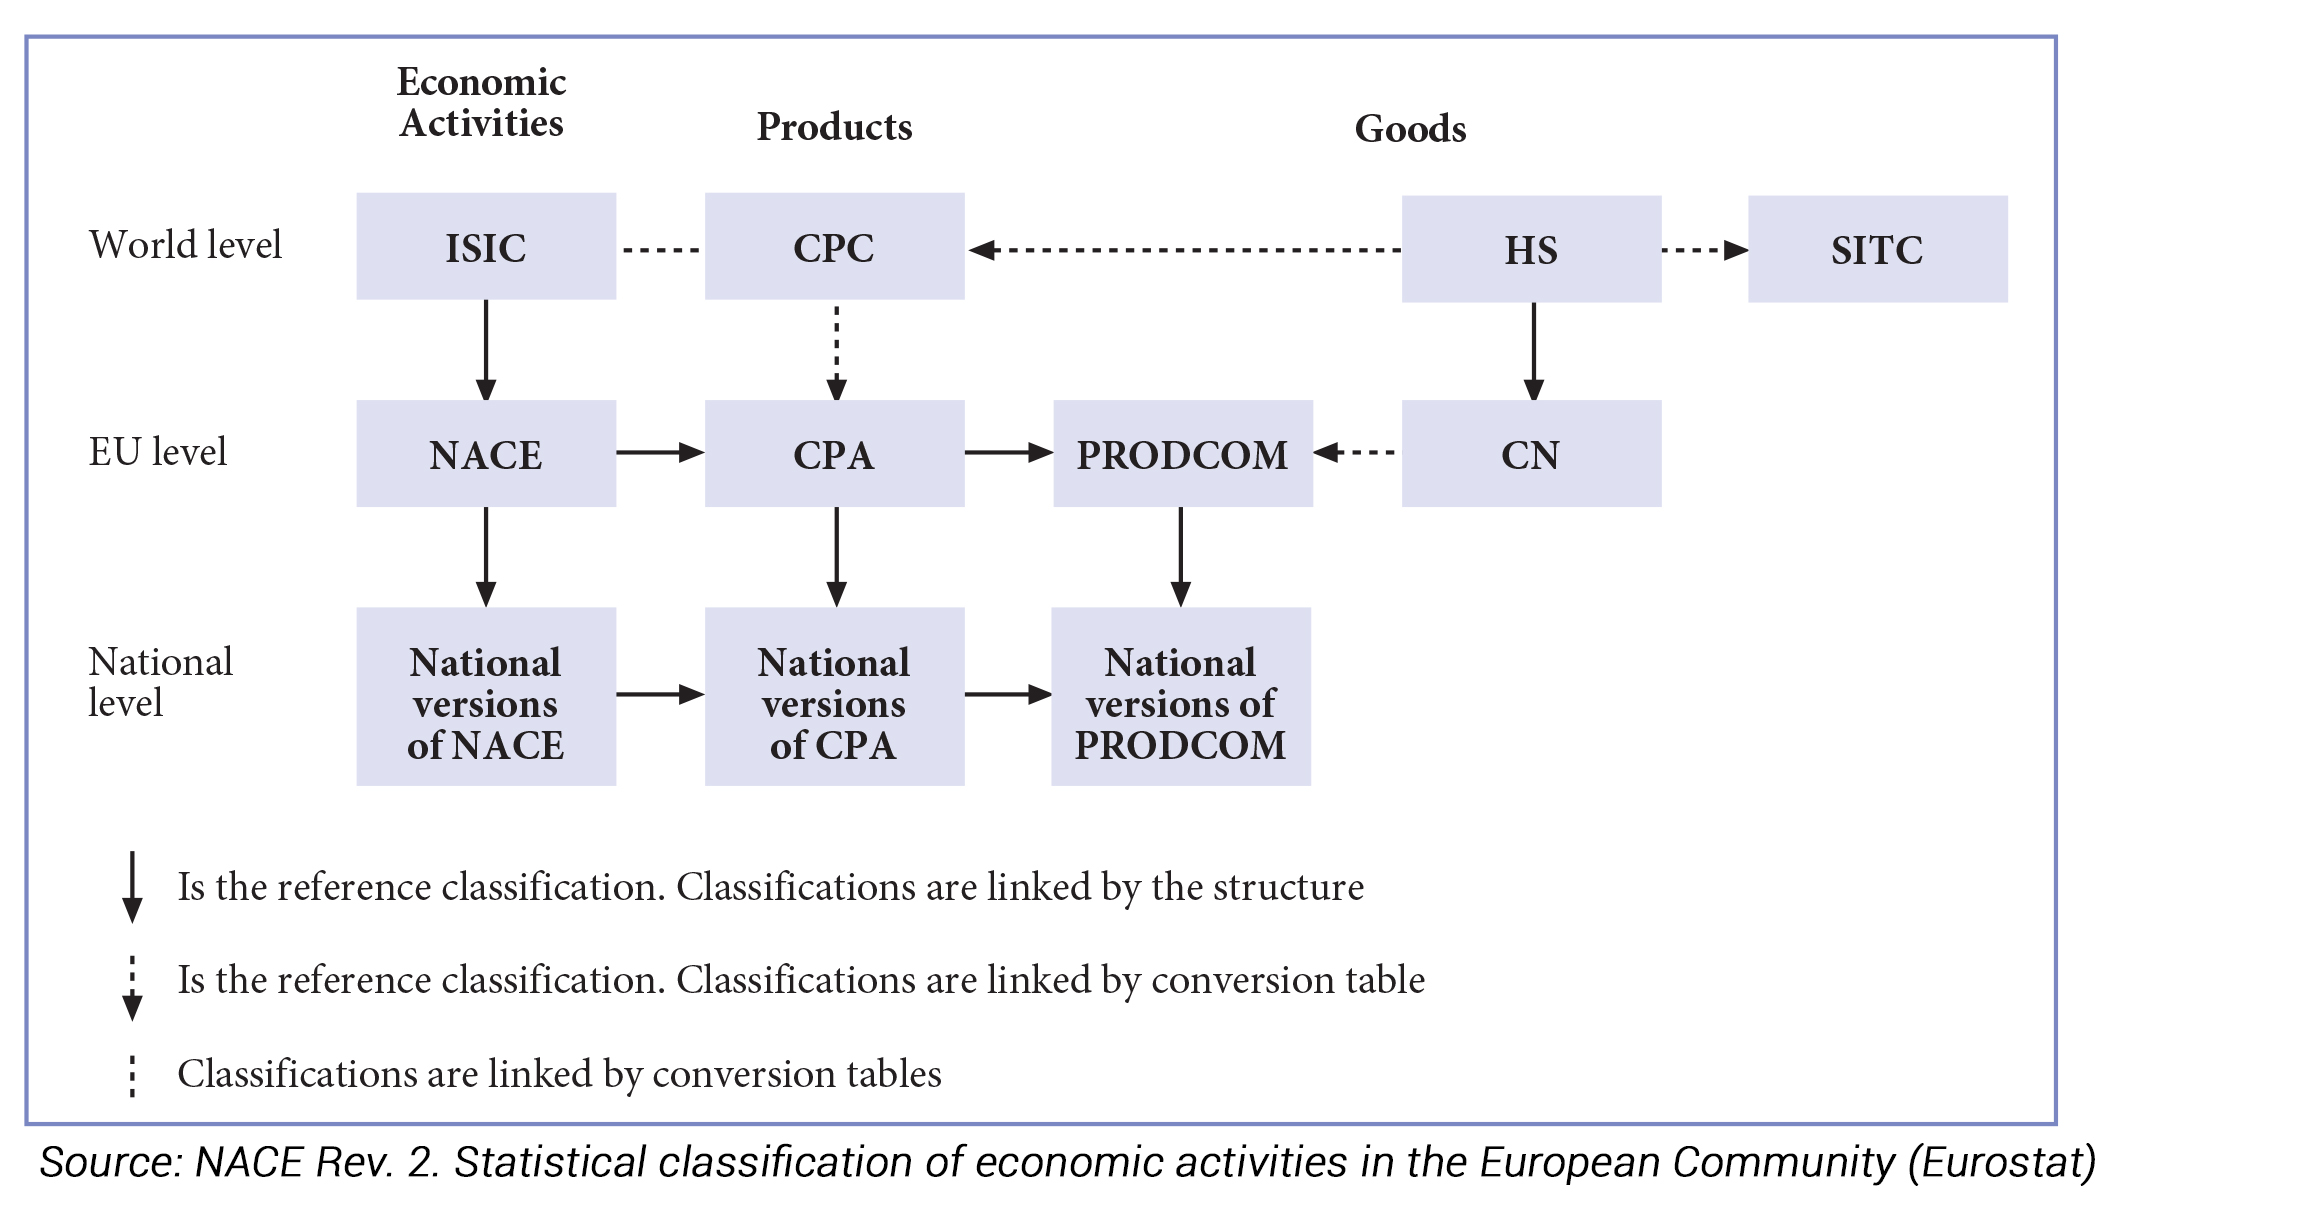
\includegraphics[width=32in]{plots/KS-RA-07-015-EN.PDF-15_p13_economic_classifications}

Within Europe, there may be slight national modifications of NACE, or
even the IOT definition. For example, Switzerland uses IOTs that are in
most applications work perfectly well with our functions, as the
country-specific modification is extremely unlikely to enter any real
life application, but still, it is not fully harmonized with the
Eurostat format and it must be imported manually from Excel
spreadsheets. Outside of Europe, a case-by-case adjustment is usually
very straightforward. Differences from ISIC and CPC are marginal and
easy to reconcile. In the future, we will add a tutorial on such a
manual adjustment, but with an understanding of IOTs, this should not be
a problem for a knowledgable user.

A case-by-case adjustment with an R code can keep the research flow
reproducible, but with coding input. In future releases we will look for
other large data sources for extending the functionalities of the
importing functions \texttt{iotables\_download} and
\texttt{iotable\_get} for the data structuring, formatting and labelling
idiosyncraticities from non-European data sources that contain more than
one country's tables.

\hypertarget{acknowledgments}{%
\subsection{Acknowledgments}\label{acknowledgments}}

We would like to express our thanks for Richard Wild again for the
helpful UK 2010 data validation.

LL and PK were supported by Academy of Finland (decisions 295741,
345630).

\hypertarget{references}{%
\section*{References}\label{references}}
\addcontentsline{toc}{section}{References}

\hypertarget{refs}{}
\begin{CSLReferences}{1}{0}
\leavevmode\hypertarget{ref-antal_slovenskom_hudobnom_2019_en}{}%
Antal, Daniel. 2019. {``{Slovak Music Industry Report} {[}{Správa} {o
slovenskom hudobnom priemysle}{]}.''}
\url{https://doi.org/10.17605/OSF.IO/V3BE9}.

\leavevmode\hypertarget{ref-R-regions}{}%
---------. 2021. \emph{Regions: Processing Regional Statistics}.
\url{https://regions.dataobservatory.eu/}.

\leavevmode\hypertarget{ref-R-iotables}{}%
---------. 2022. \emph{Iotables: Reproducible Input-Output Economics
Analysis, Economic and Environmental Impact Assessment with Empirical
Data}. \url{https://iotables.dataobservatory.eu/}.

\leavevmode\hypertarget{ref-un_iot_handbook_2018}{}%
Beutel, Joerg, Simon Guerrero, Satoshi Inomata, Soren Larsen, Brian
Moyer, Isabelle Remond-Tiedrez, José M. Rueda-Cantuch, et al. 2018.
\emph{Handbook on Supply and Use Tables and Input-Output Tables with
Extensions and Applications}. Edited by Sanjiv Mahajan. Vol. 1. Studies
in Methods, F 74. New York: United Nations.

\leavevmode\hypertarget{ref-R-rsdmx}{}%
Blondel, Emmanuel. 2021. \emph{Rsdmx: Tools for Reading SDMX Data and
Metadata}. \url{https://CRAN.R-project.org/package=rsdmx}.

\leavevmode\hypertarget{ref-botric_identifying_2013}{}%
Botrić, Valeria. 2013. {``Identifying Key Sectors in Croatian Economy
Based on Input-Output Tables.''} Ekonomski institut - The Institute of
Economics.
\url{http://www.eizg.hr/Download.ashx?FileID=010e9ee3-e20a-4d41-a59d-d65fd3d400cf}.

\leavevmode\hypertarget{ref-dhernoncourt_io_2011}{}%
D'Hernoncourt, J, M Cordier, and D Hadley. 2011. {``Input-Output
Multipliers -- Specification Sheet and Supporting Material, Spicosa
Project Report.''} Brussels: Université Libre de Bruxelles -- {CEESE}.
\url{http://www.coastal-saf.eu/output-step/pdf/Specification\%20sheet\%20I_O_final.pdf}.

\leavevmode\hypertarget{ref-02006R1893}{}%
EUR-Lex. 2006. {``Regulation ({EC}) No 1893/2006 of the European
Parliament and of the Council of 20 December 2006 Establishing the
Statistical Classification of Economic Activities {NACE} Revision 2 and
Amending Council Regulation ({EEC}) No 3037/90 as Well as Certain {EC}
Regulations on Specific Statistical Domains (Text with {EEA}
Relevance).''} \emph{Official Journal} L 393 (1).
\url{http://data.europa.eu/eli/reg/2006/1893/2019-07-26}.

\leavevmode\hypertarget{ref-32008R0451}{}%
---------. 2008. {``Regulation ({EC}) No 451/2008 of the European
Parliament and of the Council of 23 April 2008 Establishing a New
Statistical Classification of Products by Activity ({CPA}) and Repealing
Council Regulation ({EEC}) No 3696/93 (Text with {EEA} Relevance).''}
\emph{Official Journal} L 145 (65).
\url{ttp://data.europa.eu/eli/reg/2008/451/oj}.

\leavevmode\hypertarget{ref-eurostat_cpa_introductory_2008}{}%
Eurostat. 2008a. {``{CPA} 2008 Introductory Guidelines.''} {Eurostat}.
\url{https://ec.europa.eu/eurostat/documents/1995700/1995914/CPA2008introductoryguidelinesEN.pdf/df1e8d19-1156-4a1c-b384-4f95a12515e5}.

\leavevmode\hypertarget{ref-eurostat_nace_rev2_2008}{}%
---------. 2008b. \emph{{NACE} Rev. 2. Statistical Classification of
Economic Activities in the European Community}. Methodologies and
Working Papers. Luxembourg: Office for Official Publications of the
European Communities.
\url{https://ec.europa.eu/eurostat/documents/3859598/5902521/KS-RA-07-015-EN.PDF}.

\leavevmode\hypertarget{ref-ghosh_1958}{}%
Ghosh, A. 1958. {``Input-Output Approach in an Allocation System.''}
\emph{Economica} 25 (97): 58--64.
\url{http://www.jstor.org/stable/2550694}.

\leavevmode\hypertarget{ref-eurostat_r_package}{}%
Lahti, Leo, Janne Huovari, Markus Kainu, and Przemyslaw Biecek. 2017.
{``Eurostat r Package.''} \emph{R Journal} 9 (1): 385--92.
\url{https://journal.r-project.org/archive/2017/RJ-2017-019/index.html}.

\leavevmode\hypertarget{ref-leontief_io_1951}{}%
Leontief, Wassily W. 1951. {``Input-Output Economics.''}
\emph{Scientific American} 185 (October): 15--21.
\url{https://doi.org/10.1038/scientificamerican1051-15}.

\leavevmode\hypertarget{ref-R-ioanalysis}{}%
Wade, John, and Ignacio Sarmiento-Barbieri. 2020. \emph{Ioanalysis:
Input Output Analysis}. \url{http://www.real.illinois.edu}.

\leavevmode\hypertarget{ref-R-datamart}{}%
Weinert, Karsten. 2014. \emph{Datamart: Unified Access to Your Data
Sources}. \url{https://CRAN.R-project.org/package=datamart}.

\end{CSLReferences}

\end{document}
